% This is the Reed College LaTeX thesis template. Most of the work
% for the document class was done by Sam Noble (SN), as well as this
% template. Later comments etc. by Ben Salzberg (BTS). Additional
% restructuring and APA support by Jess Youngberg (JY).
% Your comments and suggestions are more than welcome; please email
% them to cus@reed.edu
%
% See http://web.reed.edu/cis/help/latex.html for help. There are a
% great bunch of help pages there, with notes on
% getting started, bibtex, etc. Go there and read it if you're not
% already familiar with LaTeX.
%
% Any line that starts with a percent symbol is a comment.
% They won't show up in the document, and are useful for notes
% to yourself and explaining commands.
% Commenting also removes a line from the document;
% very handy for troubleshooting problems. -BTS

% As far as I know, this follows the requirements laid out in
% the 2002-2003 Senior Handbook. Ask a librarian to check the
% document before binding. -SN

%%
%% Preamble
%%
% \documentclass{<something>} must begin each LaTeX document
\documentclass[12pt,twoside]{reedthesis}
% Packages are extensions to the basic LaTeX functions. Whatever you
% want to typeset, there is probably a package out there for it.
% Chemistry (chemtex), screenplays, you name it.
% Check out CTAN to see: http://www.ctan.org/
%%
\usepackage{graphicx,latexsym}
\usepackage{amssymb,amsthm,amsmath}
\usepackage{longtable,booktabs,setspace}
\usepackage{chemarr} %% Useful for one reaction arrow, useless if you're not a chem major
\usepackage[hyphens]{url}
\usepackage{rotating}
\usepackage{natbib}
% Comment out the natbib line above and uncomment the following two lines to use the new
% biblatex-chicago style, for Chicago A. Also make some changes at the end where the
% bibliography is included.
%\usepackage{biblatex-chicago}
%\bibliography{thesis}


%package used to write code snippets in rust.
\usepackage{listings, listings-rust}


\lstset{
  language=Rust,
  style=colouredRust,
}



% \usepackage{times} % other fonts are available like times, bookman, charter, palatino

\title{My Final College Paper}
\author{Sebastian Andrada Ottonello}
% The month and year that you submit your FINAL draft TO THE LIBRARY (May or December)
\date{May 2024}
\division{Mathematical and Natural Sciences}
\advisor{Charles McGuffey}
%If you have two advisors for some reason, you can use the following
%\altadvisor{Your Other Advisor}
%%% Remember to use the correct department!
\department{Computer Science}
% if you're writing a thesis in an interdisciplinary major,
% uncomment the line below and change the text as appropriate.
% check the Senior Handbook if unsure.
%\thedivisionof{The Established Interdisciplinary Committee for}
% if you want the approval page to say "Approved for the Committee",
% uncomment the next line
%\approvedforthe{Committee}

\setlength{\parskip}{0pt}
%%
%% End Preamble
%%
%% The fun begins:
\begin{document}

\maketitle
\frontmatter % this stuff will be roman-numbered
\pagestyle{empty} % this removes page numbers from the frontmatter

% Acknowledgements (Acceptable American spelling) are optional
% So are Acknowledgments (proper English spelling)
\chapter*{Acknowledgements}
I want to thank a few people.

% The preface is optional
% To remove it, comment it out or delete it.
\chapter*{Preface}
This is an example of a thesis setup to use the reed thesis document class.



\chapter*{List of Abbreviations}
You can always change the way your abbreviations are formatted. Play around with it yourself, use tables, or come to CUS if you'd like to change the way it looks. You can also completely remove this chapter if you have no need for a list of abbreviations. Here is an example of what this could look like:

\begin{table}[h]
	\centering % You could remove this to move table to the left
	\begin{tabular}{ll}
		\textbf{ALU}    & Arithmetic Logic Unit                 \\
		\textbf{CISC}   & Complex Instruction Set Computer      \\
		\textbf{CPU}    & Central Processing Unit               \\
		\textbf{GUI}    & Graphical User Interface              \\
		\textbf{ISA}    & Instruction Set Architecture          \\
		\textbf{RISC}   & Reduced Instruction Set Computer      \\
		\textbf{RISC-V} & Reduced Instruction Set Computer Five \\
	\end{tabular}
\end{table}


\tableofcontents
% if you want a list of tables, optional
\listoftables
% if you want a list of figures, also optional
\listoffigures

% The abstract is not required if you're writing a creative thesis (but aren't they all?)
% If your abstract is longer than a page, there may be a formatting issue.
\chapter*{Abstract}
Computer Systems is a critical field of computer science, but it can also have a rather harsh introduction for undergraduate students. Many of them go into introductory Computer System courses with little to no experience in lower-level programming languages, nevermind any assembly, and while one can learn well enough how a computer microprocessor functions over the first few weeks, it may be quite a while until they grow familiar with the way informations flows through a chip to make the execution of computer programs possible.

In order to help such students gain a more intuitive understanding of CPUs as they are taught in introductory Computer Systems courses, I have developed a CPU simulator made explicitly for educational purposes. The simulator focuses on simplicity, ease-of-use, and transparency: Its primary goal is not to execute assembly-code programs, but rather to cleanly display its own internal state while doing so and be easy to interact with. It gives potential users the opportunity to not only write and run their own low-level assembly code programs, but to then also watch them in action; or, is a user is interested in a particular feature of CPUs, they can see how that feature is used in a variety of different scenarios. The goal of the simulate is not to teach how a CPU works on its own, per se, but rather to function as an interactive tool that can supplement existing instruction.

\chapter*{Dedication}
You can have a dedication here if you wish.

\mainmatter % here the regular arabic numbering starts
\pagestyle{fancyplain} % turns page numbering back on

%The \introduction command is provided as a convenience.
%if you want special chapter formatting, you'll probably want to avoid using it altogether

\chapter*{Introduction}
\addcontentsline{toc}{chapter}{Introduction}
\chaptermark{Introduction}
\markboth{Introduction}{Introduction}
% The three lines above are to make sure that the headers are right, that the intro gets included in the table of contents, and that it doesn't get numbered 1 so that chapter one is 1.

% Double spacing: if you want to double space, or one and a half
% space, uncomment one of the following lines. You can go back to
% single spacing with the \singlespacing command.
% \onehalfspacing
% \doublespacing

Computer Systems is the study of the physical, metal-and-silicon devices that make up a functioning computer, and how they operate at their lowest level; these devices are the final backbone of just about any work done on a modern computer, and the field is therefore well worth exploring.

Of the countless pieces of hardware to study and delve into within this field, the CPU (Central Processing Unit) can be argued to be the most essential one. It is the heart of any computer, the piece that actually carries out the programs and computations that it was built for. It comes as no surprise, then, that most college-level Computer Systems courses begin by taking a close look at the inner workings of a simple CPU, so that they can then begin to understand how the other components of a computer support its functionality, and how it can produce computation out of just an assembly program, wires, and logic gates. Learning of this is all well and good, but getting hands-on experience with the topic is harder than one might expect: The powerful CPUs in the personal computers of students run on are all closed-source designs that obfuscate how they carry out their instructions; and even if they were transparent, the sheer breadth and depth of modifications they employ to get the performance they do would make their design completely indecipherable to a novice.

Therefore, the aim of this project is to develop a pedagogical simulator program, developed in the Rust programming language and capable of running on modern computers, that simulates a simple RISC-V CPU at the hardware level, running assembly code and then transparently displaying how the code and computed information traverse the inside of the processor. While simple, the simulated CPU implements a 5-stage pipeline design similar to the ones that are mandatory for modern CPUs. The project also seeks to include some user-facing features, like a graphical interface and the ability to step through and rewind through the execution of a program, to make the simulator more intuitive to use.

The results are promising, but with room for improvement. Certain useful features have been deemed to be beyond the scope of the current project, but the finished simulator supports the 32-bit RISC-V Base Integer specifications, and features a GUI, support for user-inputted programs, and rewinding capabilities for its ease of use as well.

\chapter{Background}
\section{An abstract view of how a CPU functions}
In order to build and understand the design of a CPU, we must first understand what it, in general terms, does. We've already established that a CPU carries out a program consisting of instructions from its ISA. However, what exactly do those instructions demand the CPU do, and what does the CPU have access to to carry it out?

We will go over the exact design of the model of CPU shown here later, with all of its intricacies and small parts. But, in broad terms, the CPU has access to: an \textbf{Instruction Memory}, where the program to be executed is stored instruction-by-instruction. A \textbf{Decoder} that reads this raw instruction, made of bits, and gleans the important details from it, like what instruction it is, what the inputs and outputs are, or other instruction-specific data. A \textbf{Register Memory}, which holds a small amount of numbered registers that store information; think of them as set mini-variables built directly into the CPU that it has quick and easy access to. A \textbf{Data Memory}, external and much larger than the previous two, in which to store larger values; and finally an \textbf{ALU}, Arithmetic Logic Unit, which is simply capable of performing arithmetic operations on the values it is given.

This explanation leaves out many crucial components and smaller parts that make the whole thing possible, but they're enough to understand the CPU's general plan, detailed here below. Note that this plan, and the designs described later, do not accurately describe all CPUs; rather, it is a simple design that, despite that, is fully equipped to execute base RISC-V programs. (REDO AS FOOTNOTE?)

1. Read the first instruction from the Instruction Memory.\textbf{(IF: Instruction Fetch)}

2. Decode the fetched instruction into useful information: The operation to be performed, the registers to be used, etc. \textbf{(ID: Instruction Decode)}

3. Read the values of whichever registers the instruction calls for from the Register Memory. \textbf{(ID: Instruction Decode again.)}

4. Perform whichever arithmetic operation the instruction calls for, using values from the registers or from the instruction itself as input. \textbf{(EX: Execute)}

5. If the instruction calls for a value to be read from or stored to the Data Memory, do so. \textbf{(MEM: Memory)}

6. Write back the end-result value of the instruction into the destination register it specified. \textbf{(WB: WriteBack)}

These six repeating steps are enough to accomplish everything that base version of RISC-V calls for, shockingly! It is enough for the CPU to successfully run low-level programs. How these simple instructions build up to the complex operating systems and graphical applications that most are familiar with today is beyond the scope of this project, but the important thing is that it is enough.

Do note that the dividing of the process of executing one instruction into six steps is entirely arbitrary; in fact, you may have noticed that the steps have been given titles in bold, but steps 2 and 3 are both lumped into the same "ID" name; These names are called "stages", and my 6 steps and the 5 stages are both arbitrary. You could subdivide this exact same process into less or more parts depending on how deep you look. However, this arbitrary model of "stages" is going to be incredibly helpful to implementing the pipeline design/feature of this simulator, which will be described later.

There are many simplifications and concerns ignored in this explanation, but one is particularly important to the CPU's design, relating to steps 1 and 2. In the modern day, we want multiple CPUs of different designs to all be capable of running the same machine code. How does the CPU know which set of bits correspond to which instruction? How does it knows which operations its designers should ensure it can compute?

\section{What is an ISAs?}

These questions all have the same answer; and so does an entirely different question, one you might've asked yourself back in the introduction: What does it even mean that a CPU is \textit{RISC-V}?

The answer is, ISAs. ISAs are how CPUs know how to read machine code not specifically tailored to them; and RISC-V is one of many ISAs, belonging to the RISC family of design. So, what are they?

Starting from the top, ISA stands for Instruction Set Architecture; you may have also heard it reffered to as just a CPU's "architecture", or of popular ISAs like x86 and ARM. We will go into the details later, but for now an ISA is simply a list of machine-code instructions that a CPU can carry out: These instructions are things like basic arithmetic operations (addition, subtraction, etc), calls to load or store data from the memory, or even jump instructions to alter the flow of the program; it specifies how to decode any machine-code instruction, stored as a set of bits, exactly. Ultimately, a program is just a list of these instructions, one after the other, that the CPU executes in order.

The ISA also contains certain hardware specifications that the CPU should be assumed to have: Things like the amount of registers available and how large a value they can store, or how the program counter ought to be measured, or even certain demands to make life easier for programmers. For example, the MIPS ISA demands that the 0th register, "Register r0", be hardcoded to the value zero at all times, so that programmers have easy access to the value and to give the option of a null register to point an instruction's destination at when its result is unwanted \footnote{\cite{waterman}}. While centered around the instructions, these additional demands are a glimpse into how important and widespread the ISA is in a CPU's design; RISC-V's specifications will be described later.

A CPU is considered to use a certain ISA if it supports and has implemented all of its instructions. ISAs were created for the goal of hardware compatibility: As long as two different CPUs made by competing manufacturers both use the same ISA, any low-level program will run on both processors because they both guarantee that they'll support the same instruction set, no matter how different their underlying design is.

Ultimately, an ISA is a standard for how a CPU should take any given line of code from a low-level program - encoded as an integer in binary, this close to the hardware - and translate that into an actionable operation that the CPU should execute when it reaches that part of the program.

\section{Why RISC-V?}
Though the ISA doesn't ascribe an exact design for how its demands should be met(that's called the \textit{implementation}, and is the domain of the CPU's manufacturer), it so heavily shapes the CPU's capabilities, and therefore indirectly its design, that choosing which ISA to implement is the most important decision one can make when designing a CPU, whether it's real or virtual. As alluded to in the introduction, there are multiple ISAs to choose from, and many more popular ones than RISC-V. So, what makes competing ISAs so different from one another, and why choose RISC-V for this project instead of any of the more popular options?


RISC-V is a modern ISA, albeit one that has not yet experienced widespread success; while it very rapidly growing in use, its two contemporaries, x86 and ARM, dominate the Personal Computer CPU and Mobile CPU market entirely for the time being. And yet, RISC-V has two major advantages over them that make it the ideal choice for this simulator.

The first is, simply, that RISC-V is fully open source. Unlike its two proprietary cousins, the full listings of all the RISC-V instructions are freely available, with details on what behavior is expected of each instruction and exactly how to glean an instruction's parameter from its 32-bit integer representation. Working with open-source sorftware and specifications is good by its very nature in that its development benefits everyone, not just its creators, but it's also a better choice practically.

The second difference is that RISC-V is a RISC ISA, while x86 is a CISC ISA; it's even in the name. These stands for \textit{Reduced Instruction Set Computer} and \textit{Complex Instruction Set Computer} respectively, and they are opposing schools of design for an ISA. The difference ultimately comes down to how many different instructions the ISA lists out: The idea of a CISC ISA is that by providing a very large variety of different instructions, most individual things you'd want a program to do can be performed with just one instruction each. By contrast, a RISC ISA aims to keep its total number of instructions low: While this would mean that code would need more total instructions to accomplish the same task, the idea is that keeping the demands simpler would allow RISC processors to have faster and more efficient designs that offset this cost \footnote{\cite{denning}}. This also coincidentally makes RISC processors a much better example for students to study, while still remaining a modern architecture that's growing in widespread use.


\section{RISC-V Instructions}

It is also enough to get a rough idea of how any given RISC-V instruction is carried out. The full list of instructions can be found on the official \textit{RISC-V Instruction Set Manual} that is freely available online, or on a number of more user-friendly guides like msyksphinz's \textit{riscv-isa-pages} \footnote{\cite{waterman}} \footnote{\cite{msyksphinz}}. A list of all the instructions in the most basic version of RISC-V, the RV32I Base Integer Instruction Set, can be found in the first chapter of the aforementioned RISC-V manual, but these instructions are broadly divided into the following four categories by the \textit{RISC-V Instruction Set Manual}:


\textbf{Register-Register Computation:} These instructions take two registers as input, perform some sort of operation on their two values (an arithmetic operation like addition, or a logical operation like a bitwise AND or NOT), and store the result in a third register.

\textbf{Register-Immediate Computation:} These are the same as RR (Register-Register) instructions, but take as input one register and one hard-coded value that's written directly into the program, called an Immediate. It's the difference between "z = x + y" and "z = x + 3".

\textbf{Load/Store:} The purpose of these instructions are simply to interact with the Data Memory, either storing a value to a specific address or reading a value from it.

\textbf{Control Transfer:} Instructions that call for the CPU to move on to a place in the code that is NOT the next instruction, potentially. These are what make the If-Then statements and Loops of high-level programming languages possible. These work because there is a simple \textbf{Program Counter}, PC, attached to the Instruction Memory that simply keeps track of which instruction should be performed next.

Each of these instructions in these categories, conveniently, move through the 5-stage process in roughly the same way based on their category.

\textbf{RR Computation:} Run through the steps as usual, feeding the value of its two input registers as the input for the ALU. ignore step 4, MEM, since Comptutational Instructions do not interact with the Data Memory.

\textbf{RI Computation:} Same as RR; but only one register is read at step 2. the other input value is the immediate, which the Decoder reads from the instruction itself.

\textbf{Load:} Load Instructions have a Register and an Immediate as input, representing the address in data memory to read from, as well as a destination register. They run through all of the steps; in the EX stage, the register value and immediate are added together to get the final address, which is then fed to the Data Memory in the MEM stage. Finally, the data loaded from Data Memory is stored in the destination register.

\textbf{Store:} Store Instructions are similar to Load, but have two registers and an Immediate, with no destination register. The first register + Immediate are the address as usual, but the second register holds the value that is to be stored into memory; and is sent directly to the Data Memory through its own special wire.

\textbf{Control Transfer:} Control Transfer Instructions have an Immediate that describes where the program should jump to, and possibly some registers. They run normally until the EX stage: Here, rather than operate on registers, the ALU is given the Immediate and the current value of the PC, which are added together to determine the Jump location. Some additional computation may be performed in this stage, such as a comparison between registers, and for some instructions the jump destination is written to an output register, but the CPU, at this point, goes back to the IF stage while editing the value of the Program Counter to complete the jump.

Do note that these categories are loose and arbitrary, to an extent. the RISC-V Instruction Manual itself has six "Types" it divides its instructions into, but these have less to do with what the instruction accomplishes and more with the details of how the CPU should read its immediates bits. The categories described above help give a broad overlook of what sort of instructions the RISC-V ISA expects CPU implementations to handle.

There are also a handful extra instructions in the RV32I that only make sense in the context of an operating system that a program would be running on top of, used for things like system calls, debugging, and accessing privileged hardware timers. Since this simulator supposedly runs its programs bare-metal with no OS beneath it, these instructions are useless in the context of the project and will not be supported.

\section{RISC-V Hardware Specifications}

Despite what was stated earlier, the ISA  does also makes certain demands, or specifications, for the hardware of the CPUs that implement it. Generally, the hardware side of things is the CPU's job, not the ISA; but in order to be compatible with every CPU running under it, an ISA needs to have certain guarantees. What is a RISC-V program tries to write a value to register "r19", but the CPU running it has only 16 registers?

RISC-V has two base variations to pick from, The \textit{RV32I Base Integer Instruction Set} and the \textit{RV64I Base Integer Instruction Set}. It also has many optional extensions, which are part of why RISC-V can have a simple core while remaining viable for commercial applications. However, it is the Base Integer Instruction Sets, reffered to as RV32I and RV64I respectively from now on, that determines hardware specification, so that is what we will look at now.

RV32I calls for a total of 32 registers. Registers r1 through r31 are general-purpose registers, each capable of holding a 32-bit-wide integer value. r0 is a special register hardwired to the constant value 0, which is useful for many situations .

It specifies that each Instruction should be 32-bits in length, though it doesn't specify how many Instructions the Instruction Memory should be able to hold. And, while the ISA doesn't make any demands of the Data Memory, and actually warns that the environment a program is executed in (like, say, an Operating System) gets to decide which parts of the Data Memory it can access, the amount it can access is upper-bound by the addresses that the RV32I Load and Store instructions can incode in their 32 bits \footnote{\cite{waterman}}.

RV64I is rather similar, with the difference that the 32 registers have a width of 64 bits each, and that Instructions themselves are 64-bits long \footnote{\cite{waterman}}.

The RV32I is simpler, and easier to understand at a glance, making it a better choice for an educational simulator.

\section{A more detailed look of how a CPU functions}

This information is enough to build a full hardware model of the CPU that the simulator will use; at least if Pipelining is ignored for now. The following is a visual representation of this model:

(INSERT DIAGRAM HERE)

Most of the components shown here have already been explained earlier, albeit with some modifications and additions. It should be noted that the components are arranged from left to right in the order of the stages; with the wires of the WB stage looping back to where the outputs should be stored. The notable changes are as follows:

1. The decoder is actually two components: The Decoder and the Immediates Decoder. The Decoder focuses on getting the indices of the two input registers and the destination register; and then a set of values called the opcode, funct3, and funct7. These are 8-bit, 3-bit, and 7-bit numbers respectively that, together, describe which exact instruction it is. The Immediates code gets the opcode in order to get the immediates out of the instruction; depending on the exact instruction, the immediate is found in different bits; RR instructions have no immediates at all.

2. There is a Branch Comparator component alongside the ALU. This allows Branch instructions to, while the ALU is busy computing the final destination of the jump, calculate whether the jump should happen or not.

3. Lastly, there are multiplexors, drawn as (INSERT INFO HERE), throughout. These simply take multiple inputs and, based on the state of the CPU, decide which one should pass through. For example, the two multiplexors right before the ALU need to decide to let the values from registers r1 and r2 pass on an RR instruction, but let the current PC and the Immediate pass in during a Control Transfer instruction.

This is enough to understand the CPU simulator, for the most part; rather than simply take in a machine-code program and execute it as efficiently as possible, which would be trivial to do in a modern high-level programming language, the simulator represents each of these components individually as structs, so that the flow of data through the CPU circuits can be displayed accurately.

\chapter{CPU and Simulator Design}

Before looking at the build of the actual CPU simulator program, it is worth going over one, in particular, of the features that this simulator seeks to implement.

\section{Pipelining}

This feature, Pipelining, must be described first: It is not a feature of the simulator as much as it is a feature of the CPU itself that this program simulates, and the design of the CPU itself must be majorly altered in order for it to be successfully implemented. However, this feature is quite powerful, and used near-universally in RISC-V CPU designs (CITATION NEEDED), and so the simulator is made with it in mind. One could describe the pipelined design to this simulator's main feature.

The previously-described CPU design has one simple issue: It is painfully slow. This design is capable of executing one instruction per cycle: one instruction per full use of each of the CPU's parts. This may seem good, but at any given moment, most of the CPU is actually going unused: The decoder is waiting on the instruction memory to fetch the instruction it needs to decode, which is waited upon by the register memory that needs the register indices to fetch their data, which is waited upon by the ALU that wants its inputs, so on.
When, say, the ALU is firing and computing, the data memory, decoder, instruction memory, and so on are all entirely dormant. They could, theoretically, be doing something useful at the same time; but because our design handles one instruction at a time, the components before the ALU have already done their part and the components after the ALU are waiting on it to finish and present its output. Theoretically, one could be multiplying efficiency of this CPU many times.

(DIAGRAM HERE OF THE STEPS, SHOW WASTED SPACE )

The solution is simple in theory, though difficult in execution: have the CPU be performing multiple instructions at once. Five of them, to be exact. This is where the five stages come into play: each stage does its part, performing its needed function for the current instruction; but when that instruction is passed off to the next stage, rather than waiting around for the full round trip, it's already receiving the information for the next instruction right away. If the WB stage is executing instruction number 9, the MEM stage is executing instruction 8, and the EX is executing instruction 7, so on.

(FOOTNOTE??)

(DIAGRAM HERE OF THE PIPELINED STEPS)

This is a good time to remind that the choice to subdivide this process into five stages, specifically, is entirely arbitrary. It's easy to see how two of these stages could be combined to have less-than-5 pipeline stages, or how the Instruction Decoding and Register Fetching could be separared into their own stages, but you can go much further than that: While 4 stages was the norm just three decades ago \footnote{\cite{denning}}, the now-also-outdated \textit{Pentium 4 Prescott} CPU had a whopping 31 stages \footnote{\cite{shimpi}}! And, by contrast, many newer CPUs like AMD's \textit{Jaguar} and Intel's \textit{Silvermont} have found a comfortable middle ground somewhere in the 10-15 pipeline stage range \footnote{\cite{kanter1}} \footnote{\cite{kanter2}}.  Theoretically, you'd want to split your CPU into as many pipelined stages as you possibly can; the more instructions you're running at once, the more efficiently the CPU is being utilized. There are tradeoffs and reasons for why this is not the case, which are better to describe later in this section.

Still, this is much, much faster;  in optimal conditions, the CPU can execute nearly 5 cycles in the time it would've taken it to do 1 cycle before! Sure, each of those cycles only performs one-fifth of five instructions, but the end result over a long program would still be a five-fold increase in speed!

Of course, conditions are not always optimal. A certain addition will be needed to this diagram for pipelining to be possible at all; A few smaller ones will be needed to handle new issues that arise out of pipelining specifically; and some of those new issues can only be mitigated, not avoided fully. Let's go over these.

The first modification, which makes pipelining possible on a basic level, is to handle coordination. Theoretically, if  every subcomponent of a CPU was perfectly coordinated and each of the five stages each always took the exact same amount of time to complete, one could simply set the CPU going, with a slight alteration to the PC so that it increments its program count 5 times per cycle instead of once. However, this is not the case: In real hardware, one cannot count on parts being perfectly coordinated; and some stages will take more or less time than others. The memory stage, notably, can require time to perform that is magnitudes longer than the other stages when it is required to go off the CPU and into a separate RAM stick, as is often used in more complex modern computers. (NEED FIXING/CITATION) Data memory structures even tend to have specialized on-CPU caches to minimize the need for this; it was originally intended for the CPU simulator to represent these fully as well, but this was proven to be beyond the scope of the project. Instead, the Data Memory is abstracted as a "black-box" subcomponent, which stores an array of data accessible by address through unknown means. Indeed, this entire timing aspect will be largely abstracted away in the simulator, operating entirely on the time unit of a "step" in which each of the instructions currently in the CPU advance by one stage; however, the alteration used to solve this timing issue in real hardware is so essential to the design, and additionally used in some of the solutions for smaller problems that cannot be abstracted away, that they will be included in the simulator regardless.

\subsection{The Backbone of Pipelining: Latches}

So, what is this modification? The main thing to be prevented here is that no stage of the CPU should recieve the inputs for the next instruction before it is done performing its computations for its current structure; to keep all five stages in sync. The ideal way to do this is to "hold" the outputs of each stage once they are computed, until the slowest stage completes its computations, and then release them all at once to begin the next step. This "holding" of outputs is done through the addition of a set of "Latches" to the CPU:

(INSERT CPU + LATCHES DIAGRAM)

There's one latch inbetween each CPU stage, with all of the outputs passing through said latch. They are named after the two stages they separate, with the leftmost being the "IF-ID Latch" for example. No latch is needed after WB, since that stage simply consists of delivering the instruction result to where it needs to go.
The latches are their own kind of register; in fact, "Pipeline Register" is another name for them. The latch holds one value for every wire that would pass through it, and constantly outputs said value through to the output end. Then, at the start of every cycle If the ALU's output wire read "13" before the EX-MEM latch was closed, and "4" after, the latch will continue to output "13" to the wire leading from the latch to the Data Memory until the latch is opened again. This achieves the 'holding' effect that was desired, and makes pipelining possible at all! In order to pipeline possible... (REFRESH ON HARDWARE LEVEL OF LATCH OPERATION)

This is one of the reasons why having more pipeline stages incurrs diminishing returns, along other tradeoffs: Simply put, Latches take a small amount of time to open, during which no computation can ocurr. The more pipeline stages your CPU has, the more times this needs to happen during one cycle, and the longer the cycle gets; therefore, adding more pipeline stages inherently has dimishing returns for the CPU's effiency. There are entire studies about measuring the efficiency of CPUs, and how this is impacted by design decisions such as its latch placement.

However, even with pipeline and latches in place, even with the efficiency tradeoffs in mind, there are still other issues that will arise from this feature. Ultimately, whoever wrote the code that this CPU is running did so under the fundamental assumption that the CPU executes one instruction of code after the other, sequentially, waiting to finish one instruction before beginning the next. This is not the case in our faster, pipelined CPU; and while that's fine in most cases, it isn't always. There are certain scenarios that can occur in a machine code program where, due to this false assumption, our pipelined CPU as-it-is will produce an output that is wildly different from what the program correctly should. These scenarios are called "Hazards" In order for the pipelined CPU model to be valid, it must  have some way to avoid or correct any hazards that come up! Hazards can be broadly divided into these groups:

- Data Hazards: Hazards that involve the reading and writing of data to registers.

- Control Hazards: Hazards that involve jump instructions.

(... WERE THERE MORE??)

Let's look at these hazards in more details, and at how the pipeline CPU design can be altereted to handle them.

\subsection{Data Hazards}

Data hazards are best introduced with a simple example, shown in assembly code. Assembly Code that is only one step removed from Machine Code: It's the same line-by-line instructions that deal directly with the CPU's registers and the Data Memory, for the most part, but presented in a way that is somewhat human readable instead of as rows of bits.

For this example, all you need to know is the RISC-V instruction ADDI. The instruction "addi b, a, i", where $a$ and $b$ are registers and $i$ is an immediate value, adds the contents of the $a$ register to the immediate $i$ and stores the result in register $b$. It is not unlike the line of code "b = a + 10" (FORMATTING) in a python program.

Imagine the following program snippet, where $\$r0$, $\$r1$, and $\$r2$ are registers and all registers start with the value 0.

\begin{verbatim}
addi $r1, $r0, 3
addi $r2, $r1, 4
\end{verbatim}

In a non-pipelined CPU, this program runs fine, as shown below. The steps relevant to this example are described by cycle; the IF and MEM stages do not matter to the example and will thus be skipped over.

(INSERT DATAHAZARD-NOPIPELINE FIGURE)

Cycle 2: Fetch the value of input register $\$r0$, $0$, from Register Memory.

Cycle 3: ALU executes $0 + 3$, its output is $3$.

Cycle 5: The output, $3$, is written back to the $\$r1$ register in the Register Memory.

Cycle 7: Fetch the value of input register $\$r1$, $3$, from Register Memory.

Cycle 8: ALU executes $3 + 4$, its output is $7$.

Cycle 10: The output, $7$, is written back to the $\$r2$ register.

\vspace{5mm}

The end result is a state where $\$r1$ holds the value of $3$ and $\$r2$ holds the value of $4$. This is the correct output, and what any such person would expect this code snippet to perform with the described starting conditions. However, look at what happens if we run the same code snippet through our pipelined design:

(INSERT DATAHAZARD-PIPELINE FIGURE)

Cycle 2:

\qquad Instr 1 ID:  Fetch value of input register $\$r0$, $0$, from R Mem.

Cycle 3:

\qquad Instr 1 EX: ALU excecutes $0 + 3$, output is $3$

\qquad Instr 2 ID: Fetch value of input register $\$r1$, $0$, from R Mem.

Cycle 4:

\qquad Instr 2 EX: ALU executes $0 + 4$, output is $4$

Cycle 5:

\qquad Instr 1 WB: The output, $3$, is written back to the $\$r1$ register.

Cycle 6

\qquad Instr 2 WB: The output, $4$, is written back to the $\$r2$ register.

\vspace{5mm}

This time, the end value of $\$r2$ is erroneous, $4$ instead of $7$! The pipelined CPU gives an incorrect output, and the reason boils down to this: \textbf{the output of Instruction 1 is needed for the correct input of Instruction 2, since $\$r1$ is both the former's destination register and the latter's input register}. But, Instruction 1's WB stage happens \textbf{after} Instruction 2's ID stage. In most cases, this would be fine; but not when the second instruction is trying to read from the same register that the first instruction modifies. It will happen even if these two instructions aren't directly sequential; only after the two are far enough temporally that the former's WB stage ocurrs at the same time as the latter's ID stage does it stop being an issue.

At the very least, having a program return a consistently incorrect output is unnaceptable, and we need to fix that. But, how?

\subsection{Stalling}

The first solution that might come to mind is: "Why don't we pause the CPU when a Data Hazard is incoming, so that it has time to catch up?". And, this is shockingly a decent suggestion! The idea is simple: As it is in the example, the update to $\$r1$, ocurring at the start of Instruction 1's WB stage, was needed halfway through Instruction 2's ID stage (Register acessing happens during the latter half of the ID stage, after the Decoder has gone). The red arrow in the diagram represents this desired update that needs to happen for correctness.

(DATAHAZARD-NOSTALL DIAGRAM)

So, we could just delay the execution of Instruction 2 by three cycles...

(DATAHAZARD-STALL DIAGRAM)

And now the program will execute correctly! This process, called "Stalling", can be applied dynamically, too; if a Data Hazard happens by just one stage of difference, the offending instruction only needs to be stalled one cycle. This method inherently costs us some of the efficiency that pipelining offers either way, though.

But, how is this Stalling implemented? As it is now, our pipelined CPU functions, but it will simply barrel forward without control: At the start of every CPU cycle, all the latches fire and transfer their information forward to the next stage. Luckily, we already have the perfect tool to control this flow, and it's those latches themselves!

Let's add a new functionality to our latches. As they are now, the latches are in "Transfer" mode:

\qquad \textbf{Transfer:} At the start of cycle, take the incoming currents of the previous stage and update the outgoing currents to match.

Now, let's add two other possible modes:

\qquad \textbf{Stall:} At the start of cycle, change nothing; keep the previous outgoing currents as they were.

\qquad \textbf{Bubble:} Set the outgoing currents to all-zeroes, regardless of what the ingoing currents were.

Lastly, we add a "Stall Control" subcomponent to the CPU. All it does is determine whether and how it needs to Stall for the given cycle, and  change the latches between these three states to perform the stall. Note: There is an additional fifth "Latch" in this setup, where the Stall Control hooks up to somewhere in the Program Counter circuitry. This simply allows the Stall Control to pause the Program Count's natural per-cycle increment; so long as the instructions are stalling, the program count needs to stall as well or the CPU will start skipping instructions entirely.

But, why are all these modes needed at all? Well, we cannot simply stall out the entire CPU, that is the same as if it wasn't running at all. What we need to do is allow for some instructions, those before the hazard-bearing instruction, to finish running while the rest of the program stops and waits for the desired number of stall cycles.

The Stall Control has all latches set to "Transfer" during normal operation. However, once an instruction with a Data Hazard reaches the ID stage, it alters the latch modes as follows.

(INSERT STALL CONTROL FIGURE HERE)

At this point, the EX, MEM, and WB stages hold the instructions that you do not wish to stall; those are Transfered so they can finish. The IF and ID stages are Stalled (using the PC and IF-ID Latch respectively), holding their current instructions. Lastly, the EX stage gets "Bubbled"; set to an output matching a "NOP" instruction that simply does absolutely nothing. This is quite important: if the EX stage was simply stalled as well, you'd actually start getting duplicates of the instruction immediately predecing the hazard-holding instruction inserted into the pipeline. Thanks to the bubble, harmless 'nop' instructions that alter nothing get sent out instead to fill that gap.

Once the instruction that holds the needed alteration reaches the WB stage, the Stall Control simply flips all latches to Transfer mode, and operation continues as normal. This does successfully resolve the data hazard, and fixes these correctness issues! However, it is still painfully slow, and gives up much of the advantage of pipelining anytime that a register is written to and then read from in quick succession; as it turns, this is rather common. We've already accepted that conditions will not often be optimal for pipelining, but this is a serious blow. Can we do better than that?

\subsection{Forwarding}

The answer is that yes, we can! Let's go back to our data hazard example, when it is un-stalled:

(DATAHAZARD-NOSTALL DIAGRAM)

Obviously, the issue is clear here: The data needed in the ID isn't ready until Instruction 1's WB stage, and is needed in Instruction 2's ID stage. Except, this isn't really true. Technically, that data has already been computed by the end of Instruction 1's EX stage, found in the output of the ALU. And, it is Instruction 2's EX stage that needs the data for the addition calculation, not the ID; as long as the ALU gets the correct integer input of $4$ instead of $0$, it doesn't care where it came from. So, technically, the desired data to resolve this hazard \textit{is} available by the time it's needed; it just doesn't have the pathway to get there in time. So... what if we added that pathway ourselves?

That is exactly what forwarding is! Extra data pathways are added  into the ALU input; controlled by a multiplexor that reads register indices to decide if forwarding is needed. The pathways come from the MEM-stage output if the offending instructions are adjacent, and from the WB-stage output if they are one instruction apart; any more than that, and there is no Data Hazard at all. These are called "EX-EX Forwarding" and "MEM-EX Forwarding" respectively. There is a third type of Data Hazard, which occurs when a value is loaded from the Data Memory to a register and then stored to somewhere else in the Data Memory immediately after; the store will still have the stale value from that register, from before it was read to. An extra pathway and multiplexor, from the WB stage to the Data Memory, handles that; this is called "MEM-MEM Forwarding" . With that, all of the Data Hazards are resolved, this time without performance loss!

(INSERT FORWARDING TYPES DIAGRAM)

Doesn't this make stalling entirely obsolete? Well, not exactly; there's still one more unhandled data hazard case. What if happens if a load instruction is immediately followed by an arithmetic instruction, using the register that was loaded to? (Or by a store instruction, using the register to calculate an adress rather than as the to-store data). As seen below, the data is retrieved at the end of the Load's MEM stage, yet is needed at the beginning of the EX stage so it can be used in the arithmetic operation. In this case, the data truly doesn't come soon enough!

The ideal solution is a hybrid of the two techniques: If you stall the second instruction by just one cycle, the data can now arrive just in time. It can even use the same "MEM-EX Forwarding" from earlier without any new pathways needed!

\subsection{Control Hazards}

There is a second reason why stalling, or at least the Stalling Control we implemented, is still useful: Control Hazards.

So, when do control hazards occur? Well, anytime any jump instruction is called. The problem is simple: anytime that a jump instruction occurs, the new address to jump to is already needed by start of the next instruction's IF stage: but it is calcuated in the jump's EX stage, where the ALU adds the jump value to the existing Progam Count.

This hazard is going to lose us cycles no matter what; but to mitigate that, the first step is to add another forwarding pathway from the ALU output directly to the PC in the IF Stage. This almost resolves the issue, with the jump happening at a 2-cycle delay, though there's one more problem: Inbetween the  jump instruction entering the IF stage and the jump address being calculated in its EX stage, two instructions directly after the Jump get loaded in; instructions that shouldn't run at all, since the program supposedly jumps to another location. After those two, though, the output of the EX stage gets forwarded back to the PC in the IF stage, so the solution is simple: On the cycle that the jump instruction is in the EX stage, we tell the Stall Control to set the latches of the IF and ID stages (the stages holding the two erroneus instructions), to go on "Bubble Mode". This harmlessly flushes out those two instructions before they have a chance to perform any alterations, and the instruction following them will be from the correct jumped-to address! The end result is akin to stalling the instruction following a jump for 2 cycles, in order to avoid the Control Hazard.

In fact, you could achieve the same result by stalling the instruction 2 cycles, using the method described in the earlier section on stalling. This would work: there, the two erroneous instructions never enter the pipeline at all. It would be simple if all hazards were handled through the same method, so why not just do that?

It has to do with \textit{Branching} control instructions, or Branches. A Branch is similar to a jump, but it also makes some sort of logical comparison between two inputted register value. If the comparison resolves to true, the Branch jumps to the destination; if it's false, the jump is not taken and the program continues to the next sequential instruction. Branches are the main option assembly programs have for introducing, well, branching pathways to the control flow of their code, and what compilers most heavily use when compiling if-statements and loops from high-level programming languages.

Well, as it turns out, handling jumps  with the flushing method is actually a small optimization that potentially saves time for \textit{branching} control instructions. Branching control instructions are almost the same as jump instructions: there's just an extra subcomponent in the EX stage that compares its values to check if the Branch is to be taken, which decides if the Program Count is changed or left alone. However since we cannot know whether the branch will be taken or not \textit{until} the EX stage, this causes a difference between the flushing and stalling methods: In the stalling method, the instruction after the Branch has to get stalled regardless of whether the Branch gets taken or not; it has to start stalling right away. In the flushing method, the CPU flushes and jumps as usual if the Branch gets taken; however, if it does not get taken, the Stall Control simply... doesn't do anything. Those two "erroneous instructions" are actually now the correct path forward for the program to take, and it just lets them happen. So, flushing the Branches instead of stalling them makes no diffence if the branch is taken, but saves cycles if it isn't! This method is also called the "Fetch and Cancel When Taken" method of handling control hazards, since the "cancel" or flush only happens if the Branch is taken.

\subsection{Final CPU Design}

(INSERT FIANLIZED CPU DESIGN HERE)

The final design of the CPU we will simulate is therefore as shown above. Instruction, Decoder, Registers, Arithmetic, Data Memory, and Writeback; built with the intent that the simulator will display its own internal state to a similar level of granularity as the diagram above.

The flow of instructions through the wires is separated into 5 arbitrary stages in order to \textbf{Pipeline} them for major performance boosts, with the separation enforced by a set of Latches.

Then, in order to deal with the correctness hazards that this pipelining incurrs, additional \textbf{Forwarding} pathways and a \textbf{Stall control} in the latches are implemented to sidesteps those hazards, while also minimizing the performance loss incurred.

\section{Simulator Design}

The actual simulator is a program written in the Rust programming language, and aims to faithfully replicate the operation of the CPU at the same level of abstraction used in the diagrams above! as a result, it can be compiled and run on most modern personal computers. Its final iteration fully supports the Risc-V 32-bit Base Integer Instruction Set, with the exception of system-call instructions that are meaningless without the context of an OS outside the program, and the failsafe for a particular Data Hazard that turned out to be rather difficult to impelement.

The goal of the simulator itself is simple: to take in a machine-code RISC-V program as input, set up a virtual construct in Rust that replicates the low-level, semi-abstracted model of a CPU that has been discussed in the background chapter, and then run said program through it in a way where the simulated CPU's internal state is always transparent. Other goals, such as a User Interface, are additional features and not part of the core design. This design was eventually accomplished, though the project had to go through a major restart partway.

\subsection*{First Draft}

The first draft was quite neat in theory, though rather idealistic. The core idea is to rely on the way that the diagrams above dive the CPU into separate "subcomponents", such as the Program Counter or the ALU, which only pass along information through predefined wires; this is something the final design will keep.

The core idea of the first draft is that each of these subcomponents should be represented by its own unique "struct" in Rust; despite the name, these are much closer to the Classes and Objects of Object-Oriented Programming Languages like Python and C++, made to hold a specific set of variables as well as functions tailored to those variables. Every "subcomponent" on the graph would be represented with its own unique struct: It would have variables for both every input and output connection it had with other subcomponents; and if it was a stateful subcomponent that stores data, like the Program Counter or any of the three Memories (Instruction, Register, Data), it would also have variables for recording said state. References to the structs that they need to fetch input data from, as well as functions to fetch said data and to perform the subcomponent's intended purpose complete the struct. Then, all of this would be hooked up to some sort of master "setup" and "step" functions; the former would initialize all these structs and insert the program into the Instruction Memory, while the latter would activate these structs one by one to perform a single full CPU cycle, over and over.

The advantages of such a design are apparent: The different structs are entirely separate from one another, making them easy to test on an individual level and to see the state of any one given subcomponent at a time. It also meant that the layout of the code resembled the design of the actual CPU somewhat intuitivelty.

However, this design also has two glaring flaws: The first is more manageable, and it is simply that the design's method of passing data between structs, that being of giving each struct a persistent reference to the structures that send information to it, is entirely incompatible with Rust's memory-safety failsafes. Well, the idea of doing that, in itself, is not, but the problem comes from the fact that, due to the CPU's cyclical nature, these links of one struct borrowing a refference to the previous struct eventually form a loop. The details are not relevant to this project, but using such persistent references in a loop with no clear top-level "owner" goes against the language's philosophy to the point of not being allowed at all. This issue could've been resolved on its own if it was the only problem with the design; for example, by simply having the step function handle all the wiring itself and using the subcomponent structs for their internal computations only.

That said, the second issue is that the design was unbearably repetitive, to the point of being confusing to look at. The distinct input-output variables on each struct meant that every piece of information in the CPU essentially took up two variables instead of one, and the process of computing a piece of data and sending it to the next subcomponent in the stage became a chore with many unecessary middle-man steps inbetween.

\subsection*{Final design}

The second and final iteration of the simulator took a slightly different approach, one that relies more closely on the nature of this CPU as being ultimately made of logic gates and wires, and employs style of design often used to simulate simpler logic gate machines.

The idea now is to divide the CPU design into two categories, and therefore two structs: Its State and its Logic. The State consists of all the naturally  stateful elements of the CPU as described before: The Program Counter, the three Memories, and also all of the Latches, which essentially store the supposed current state of the wires they are supposed to clamp down on. The Logic stores everything else that has no state; or, rather, it stores all of the \textit{wires}, since that is all else that matters. A subcomponent like the ALU has no internal state; it reads data of the two operands and the opcode, and calculates its output solely off of that; even to be accurately rerpesented, this representation can be done simply as a piece of code that performs the ALU's function. Even the wires are only stored in persistent variables for the sake of visually displaying the CPU's state later. So, the entirety of the CPU is separated into a State struct and a Logic struct, and each struct has an "Update" function written to it that takes the other struct as a mutable reference and  updates the state of all its own variables at once: For the State Struct, this means handling memory changes like updating the PC, enacting the write of data into the Writeback register, and Storing data into the Data Memory when Store instructions pass by. For the Logic struct, it means reading the state of latches and registers and determining what signals should be traveling through the wire as a result of their changes.

(DIAGRAM OF CPU, COLOR-CODED FOR STATE AND LOGIC MAYBE?)

This setup is so useful because it makes the actual update of a CPU cycle incredibly simple: Just run the update function for the State struct, followed by the update function for the Logic Struct. This is not entirely true, as the implementation of stalling will complicate things a little, But for the most part, this makes up the base of the simulated CPU and the process for executing one of its cycles:

\begin{lstlisting}
	struct State {
		pc : u32,
		instr_mem : Vec<u32>
		// ... more State variables
	}

	struct Logic {
		added_pc : u32,
		instruction_out : u32,
		//... more Logic variables
	}

	impl State {
		fn update(&mut self, &mut logic: Logic){
			self.pc = logic.added_pc:
			//... more State updates
		}
	}

	impl Logic {
		fn update(&mut self, &mut state: State){
			self.added_pc = state.pc + 4;
			self.instruction_out = state.instr_mem[(state.pc / 4)]
			//... more Logic updates
		}
	}

	fn step(state: &mut State, logic: &mut Logic) {
		state.update(logic);
		logic.update(state);
	}
\end{lstlisting}

This code is entirely functional as a rough base for the simulator's design; all the ,main body of the program needs to do outside of this function is to initalize the two structs, get the user-fed instruction into the instruction memory, and then run the $update(state, logic)$ function repeatedly until the program has run its course!

Other features can and will be implemented as well, of course; but, the design shown above is a sweeping generalization. It's worth taking a closer look at what the final, detailed program looks like, now that its basic structure is understood.

\subsection*{Structs and Sub-Structs}

The final design could indeed have just unceremoniously dumped all of its State and Logic variables into their respective structs; but this would've made a rather huge mess, resulted in individual wires (especially different wires that carry the same piece of data at different stages) being hard to keep track of, and would've been rather confusing and inelegant in general; this is one of the issues the first draft design sought to resolve. Therefore, the final design for the structs instead looks like this:

\begin{lstlisting}
	#[derive(Clone)]
	pub struct Registers {
		pub ifid: IFIDLatch,
		pub idex: IDEXLatch,
		pub exmem: EXMEMLatch,
		pub memwb: MEMWBLatch,

		pub pc: u32,

		pub instr_mem: Vec<u32>,
		pub reg_mem: Vec<u32>,
		pub data_mem: HashMap<u32, u32>,
	}

	//this structs holds all the wiring of each stage

	#[derive(Clone, Default)]
	pub struct Logic {
		pub fetch: IFLogic,
		pub decode: IDLogic,
		pub execute: EXLogic,
		pub memory: MEMLogic,
		pub writeback: WBLogic,

		pub pc_stall: bool,
	}
\end{lstlisting}

Rather than having a soup of variables, all of the states tied to a specific latch and all the wires tied to a specific pipeline stage are sequestered off in their own sub-struct; when used like this, these sub-structs are just fancy ways of holding variables and don't get in the way like they did in the previous design. It also allows for said sub-structs to be stored in their own file, leading to a much cleaner folder structure for the source code. In a way, these sub-structs are effectively just organizational folders for the variables within the program.

\begin{lstlisting}
use crate::components::*;

//The IF-ID Latch
#[derive(Clone, Copy, Default)]
pub struct IFIDLatch {
    pub base_pc: u32,
    pub added_pc: u32,
    pub instruction: u32,

    pub id_stall: u8, //stall, bubble, or neither?
}

impl IFIDLatch {
    pub fn bubble(&mut self) {
        self.base_pc = 0;
        self.added_pc = 0;
        self.instruction = 0;
    }
}

//holds all of the wiring of the ID stage
#[derive(Clone, Default)]
pub struct IDLogic {
    pub decode_r1: u8,
    pub decode_r2: u8,
    pub decode_opcode: u8,
    pub decode_rd: u8,
    pub decode_funct3: u8,
    pub decode_funct7: u8,

    pub regmem_r1: u32,
    pub regmem_r2: u32,

    pub immediates: u32,
}
\end{lstlisting}
(FOOTNOTE EXPLAINING THIS IS DECODE.RS)
(MAYBE DIAGRAM OF DECODE STAGE TO COMPARE?)

This is an example of one such file; in genral, everything is stored as simply as possible, with the data types one would expect: Most wires carry a 32-bit unsigned integer; since this is a 32-bit system, that is the format that the CPU preferst to handle its data in. while wires for the smalled opcode, funct-3, and funct-7 all use unsigned 8-bit integers. Technically, the latter should use u7, u3, and u7 respectively, but establishing custom-length integer data types just for them was deemed to not be a very high priority.

The instruction memory and register memory are simply represented as u32 Vectors, with the former having a length equal to the number of instructions in the program and the other having 32 integers exactly; this makes accessing registers incredibly intuitive, as the nth register can be found in $state.reg_mem[n]$. The data memory is orders of magnitude larger than the first two though, and is going to consist mostly of empty addresses, so using a vector would have been incredibly wasteful; instead, it uses a hashmap of 32-bit integers with numbered keys, matching the size of a "word" that the \textit{Store Word} and \textit{Load Word} instructions use. This means that the smaller load-store instructions need to slice off part of the accessed word, but this was fairly manageable.

It is worth noting that there are some wires which aren't often shown in CPU design diagrams, but are nonetheless present in a real CPU, and therefore in our simulation too. For example, the Forwarding Multiplexors are only shown as having the base, EX-EX, and MEM-EX register values going into them, but in reality they also read a few other values, such as the opcode and register indices of the current and next two instructions, to decide which forwarding, if any, should ocurr.

Ultimately, this makes the storing and accessing of information about the CPU pretty intuitive, which will come in very handy for the User Interface.

\subsection*{Update Functions}

Unfortunately, the two update functions aren't quite as simple. In a sense, they are: Each one goes has the struct going through all of its variables and updating them according to the internal logic of the CPU design. However, this updating needs to be done in just the right order in order to make things work properly. This is one case where building a virtual simulator is actually harder than making a real CPU: In a real CPU, all of this happens instantaenously and at the exact same time, literally within that given CPU clock cycle, and so it does not need to worry about this. But the simulated CPU runs one-step-at-a-time, and doing certain updates before others can cause massive errors. For example, the latches in the State struct's update function need to be updated in order from right to left, starting with the MEM-WB latch and ending with the IF-ID latch. Otherwise, if the IF-ID latch updates before the ID-EX latch, the information it was supposed to send directly over, like the base PC and added PC, that information vanishes for good. The problem is especially tricky with the Logic update function where, thanks to forwarding and writebacks, certain computations of a pipeline stage rely on information from a stage further to the right. Thankfully, part of the job of the latches here is to serve as a stopgap to separate the stages, so the issue is merely annoying rather than impossible.

A lot of the desired ordering was figured out, in part, by writing a large amount of test cases and catching any correctness errors, though that will be discussed in detail later.

Its ordering aside, the actual code contained within is mostly understandable, just there to perform the functions that those sub-components would in a real CPU. The decoder code takes an instruction and separates it into its relevant pieces using bit-masks and bit-shifts; the register memory writes and reads data off the 32 general-purpose registers, so on. The most crucial one is the ALU, since that's  utlimately where the actual computation of most instructions takes place, and even that one is farily simple: It takes in the two operands, looks at the opcode to figure out what sort of arithmetic operation it's supposed to perform and spits out the output to $logic.execute.alu_out$. To whomever is interested in more details, the update functions and my comments on them can be found in the $components.rs$ file, right under the structs.

\subsection*{Stalling}

There is one piece of the core simulator that doesn't fit neatly into the description above, in part because it operates above the other components. While the variables to indicate whether components are being stalled or not are stored within the State and Logic structs, the code for the Stall Control happens directly at the step function, performed after the state update but before the logic. Since forwarding is implemented, stalling is only needed for Control Hazards and for Load-ALU hazards; the former is fully implemented, while the latter, unfortunately, could not be debugged in time.

\begin{lstlisting}

pub fn step(state: &mut Registers, logic: &mut Logic) {
    //Checks if Stalling or Bubbling is needed
    //Check if a jump is performed! those always need a stall on the NEXT step
    let must_jump_stall_next = logic.fetch.jumped;

    //if there's a Load in EX stage and an ALU instruction in the ID stage,
	// using the same register...

    state.update(logic);

    //always do this inbetween!!!
	//that way the right instructions get stalled/bubbled,
	// but their logic is not allowed to propagate.
    if must_jump_stall_next {
        //If there is a jump, need to bubble IF and ID of now...
		// so the ID and EX of next step!
        logic.pc_stall = false;
        state.ifid.id_stall = 2; //bubble flag  on
        state.ifid.bubble();

        state.idex.ex_stall = 2; //bubble flag on
        state.idex.bubble();

        state.exmem.mem_stall = 0;
        state.memwb.wb_stall = 0;
    } else {
        logic.pc_stall = false;
        state.ifid.id_stall = 0;
        state.idex.ex_stall = 0;
        state.exmem.mem_stall = 0;
        state.memwb.wb_stall = 0;
    }

    logic.update(state);
}
\end{lstlisting}

I suspect that this decision to place the stall decision there is part of what made the Load-ALU stalling so difficult to figure out, and is worth addressing in future revisions. But with that, the core simulator design is complete!

\section{CPU-Simulator Features}

Of course, such a simulator as it currently stands is pretty bare-bones for the sake of educational purposes. So, in a rough order of complexity-to-implement, the following features were added to the simulator: The ability to feed the simulator a machine-code program from a text file, the ability for the simulator to store and load the entire state of the CPU in previous steps, and a simple graphical user interface that displays and clarifies the internal state of the CPU at its current cycle. But, why these three?

The goal of these features are to make the simulator easier to use, and to aid its goal of helping users attain a more intuitive understanding of a CPU's inner workings. The last feature is by far the most critical for this: The GUI displays the same information as one of the CPU diagrams from earlier, but with the actual data of a live program running through it overlayed on top; and it can be analyzed step by step! The finalized GUI for this simulator is very rudimentary and much smaller in scope than what was originally intended, but it accomplishes its intended purpose well; it will be described in more detail later.

The purposes of the other two features are supplementary in nature, but no less useful: User-Inputed programs make it possible for the end user to provide their own code and run programs tailored around whichever instructions or CPU features they are interested in getting a better grasp of rather than one sample program, without needing to edit the source code and recompile at least. The latter is pure ease-of-use, and ends up implemented solely as a way to be able to "backstep" or "rewind" the simulator at any given step, but is incredibly useful in that alone: If a user steps forward and suddenly finds themselves confused by the CPU's new state, they can rewind back to the previous cycle, or more, to refresh their memory and see how it got there.

\subsection*{Implementation of User Input and Rewinding}

These features were both pretty simple to implement, and are only described here for completeness. The User Input simply involves using Rust's built-in libraries for commandline arguments and file reading, taking in the filename and creating the Instructions vector out of the file's contents line-by-line. For the sake of simplicty, the program expects one machine-code instruction per line, formatted as a 32-bit binary integer. Originally, the project was going to accept RISC-V assembly code as input and have its own built-in assembler to translate them into the binary machine code that the simulator needs, but this has proven to be out of scope.

The backups/rewinding were only a little more involved, requiring just the creation of a "Snapshot" struct that contains one State struct and one Logic struct within it. This new struct then works as a full snapshot of the CPU's previous state: The simulator clones the current State and Logic structs at every cycle, and places the clones in a "backup" vector of Snapshots; When the user asks to go back a step, it simply pops the most recent Snapshot off the backup vector and replaces the State and Logic structs it is currently using with those within the Snapshot. Due to their simplicity, both of these features were very easy to implement!

\subsection*{Graphical User Interface}

In the initial writeup, the plan for the simulator's GUI was incredibly ambitious (the entire writeup was, but that is besides the point): The plan was to learn an application development framework such as Qt as part of the project, develop a proper graphical interface that would run its own window, and then implement all sorts of additional nice features like separate tabs for the different memories, animations to show which wires are actually passing relevant information in any given cycle, and so on. Suffice to say, this idea was entirely out of scope and would have required spending a lot of time studying something entirely unrelated to Computer Systems, and I ended up scaling back to something much more reasonable to get working quickly: An ASCII-art text interface, that can be printed directly to the commandline terminal.

(INSERT SCREENSHOT OF SIMULATOR GUI)

It's fairly dense and all but requires the user's terminal to be maximized, but it properly displays the CPU diagram and all of its relevant information! The top line displays the instruction that each pipeline stage is currently executing, in assembly; the body displays the entire CPU diagram, and the value that every wire currently holds; and the bottom shows the entire values of the register memory! The implementation, while involved and time-consuming, was mostly simple: the text-art for the diagram was drawn up using an online tool named ASCIIflow, and the $display_cpu$ function responsible for it was given a reference to the State and Logic structs, from where it could effortlessly pull the needed values for the diagram display. This simpler method also provides its own advantage: While much less sleek, the commandline approach makes the program more likely to work across operating systems without any tinkering required than an intricate app-develoment framework might.

The most involved part is actually the instruction-display at the top; in order to make it useful and human-readable, having it spit out the instructions as 32-bit binary integers would not cut it. Therefore, the GUI makes use of an additional $display_instruction$ function that converts a given machine-code instruction into its equivalent assembly, a "reverse-assembler" in a way. This feature wasn't too time-intensive, and it was a good use of my growing familiarity with the format of RISC-V's 32-bit instructions.
There is also an user-input prompt at the bottom that asks the user to either move to the next step or the previous step, completing the implementation of the rewind feature.

To my surprise, I have found this user display to be rather satisfactory of the projects needs, despite its stark contrast to the initial goal. The only missing feature that I feel is essential, but ran out of time to implement, is an extra line or two for displaying any values that the program writes into the Data Memory. It is imperative to only present modified data rather than the entire storage unit, as otherwise the sheer amount of information would be utterly useless; luckily, the formatting of the Data Memory variable as a hash-map inherently alleviates this concern. It may also be possible to replicate the desired effect of "indicating which wires are passing important information" using color-coded terminal text, but the method used to print the GUI would have made it far too time-consuming to introduce on a whim.


\chapter{Conclusion}

On the whole, this project has been a learning experience in more ways than I ever expected. I've had to start over or rethink my approach to a particular challenge multiple times, and I doubt that I would've grown as familiar with CPU architectures as I have, had I not commited so many mistakes. I would almost recommend that Computer System students give their own try at building a CPU simulator rather than just using mine, but I get the feeling that none of them have the extra free month or three to dedicate to such an endeavor. Still, I am rather proud of what I've ended up building: A simple, tightly-focused RISC-V simulator that, while lacking in the fancier features of its contemporaries, has enough graphical








%this part will go somewhere in the Conclusion, not sure where yet.
That said, there are some other potential features that could be added as future extensions to the project, even outside of the GUI.

\subsection*{Future Extensions}

The most obvious and tempting features to include are certain ones dealing with ease-of-use: A built-in RISC-V assembler, which would allow users to write and input programs in the much more human-legible format of assembly code; an english "narration" of sorts of what each stage accomplishes on a given cycle; or perhaps even the ability to edit values of the CPU on the fly in order to study how that changes the outcome.

Another approach is to extend the capabilities or fidelity of the simulated CPU. This project limits itself to a simple design and just the RISC-V 32-bit Base Integer Instruction Set  for the sake of remaining easy-to-understand for newcomers to Computer Systems, but additional support for some of RISC-V's myriad Standard Extensions could be added to give the simulator some much-needed versatility. These range from things like the inclusion of multipication instructions and floating-point numbers to vector calculations and a whole 64-bit instruction set, and would come especially handy for if anyone studying the RISC-V architecture specifically.

As far as incrasing fidelity, the obvious choice is the Data Memory. As described before, the Data Memory in this simulator is a "black box"; it takes in requests to load or store data to certain addresses, and does so without any paerticular consideration of how that is physically possible. This is technically true for our Register and Instruction Memories as well, but those are small enough that they can easily fit on the CPU chip, and thus be set up pretty similarly to what our diagram presents. This is not the case for the Data Memory: The Data Memory is magnitudes larger than either of the former two. Even if one only counts the data that a running program access with its 32-bit addresses, the Data Memory can store a mind-boggling $2^28$ Words (4-byte chunks of data) compared to the Register Memory's measly 32! That's about 4.2 gigabytes and 128 bytes, respectively; and, since the operating systems of modern personal computers want to be running many, many programs at once, the actual size tends to be even larger in practice, nowadays. Therefore, a possible extension of the simulator would be to alter it to replicate the following more realistic setup: One where the actual Data Memory is stored off the CPU chip, massive but painfully slow to access; while a series of caches mediate this access to hopefully maintain on-chip speed for the more frequently-used parts of Data Memory. This setup would allow the simulator to be usable for learnign to work with memory structures as well as CPUs, and could implement crucial features for it such as the aforementioned caches or Virtual Memory.
(CITATION NEEDED?)

If one wishes to extend the CPU with more advanced features, two relatively-simple ones that go hand-in-hand are OOE (Out-of-Order Execution) and Register Renaming.

OOE is simple in concept: Pipelined CPUs sometimes need to stall. In real hardware, CPUs sometimes need to stall a \textit{lot}, especially whenever there's any kind of cache miss in the Data Memory. And many times, multiple of the instructions immediately following one of these costly and stall-heavy instructions (like a Load to an address that's not in cache) are totally unrelated to the slow instruction; like, say, a bunch of arithmetic operations that don't interact with any of the same registers that the costly instruction does. So, why not keep the CPU running while the Data Memory is busy fetching, and get those instructions out of the way? It's out-of-order, but still correct and much faster so long as any instruction that shares registers with the slow instruction stalled out properly the whole way through; these are potential new Data Hazards that OOE brings along with it. This feature should only be implemented after the higher-fidelity Data Memory and its increased time costs, as that's where the biggest performance increase from this technique will come from. If one does this, it may be worth adding an extra piece of data display to note which instruction the Data Memory is diligently working at in the background, while the rest of the CPU continues to run. There are many involved pieces to implementing OOE, but the basic idea is to look at a "window" of the next few instructions and randomly pick one to execute that would not cause a data hazard.

Similarly, Register Renaming should only be implemented after OOE, because Register Renaming is to OOE exactly as Forwarding is to Pipelining: It is a feature that purely exists to sidestep the former's "false" Data Hazards. It goes a little like this: OOE's Data Hazards are much more expansive than Pipelining, due to it changing the ordering of instructions around, divided into three broad categories. Looking back at our earlier example:

1. if the Load instruction loads the value $13$ from memory into register $\$r1$, and then an Add-Immediate instruction right after it calculates the value $200$ into $\$r1$, the correct behavior would be for the load to finish executing, then for the add-immediate to execute for a final result of $\$r1 = 200$. However, with OOE, the ALU-using instruction would finish executing, and thus finish writing back, way before the Load, and the final value of $\$r1$ would be $13$! This is a \textbf{WAW} Write-After-Write hazard, since both instructions wrote to the same register.

2. if the Load instruction loads the value $13$ from memory into register $\$r1$, and then an Add instruction right after it adds $\$r0$ and $\$r1$ together, one would expect first $13$ to be loaded into $\$r1$, and then for the Add to add $0$ and $13$ together to store in wherever the destination register is. However, with OOE, the Add instruction will instead read whichever value was in $\$r1$ \textit{before} the Load, and produce a totally wrong addition! This is a \textbf{RAW}, Read-After-Write hazard.

3. This one requires a full re-ordering, but that is fairly common in OOE. Imafgine that the Load instruction loads its data from the address $1024(\$r3)$, with $\$r3$ currently holding 0, and that an Add-Immediate instruction after it stores its result,  $28$ to $\$r3$. It is expected that the Load instruction will load from address $1024(0)$, but if they are executed out of order, the Add-Immediate will edit $\$r3$ first and the Load instruction will load from $1024(28)$, a completely wrong address! This is a \textbf{WAR} Write-After-Read hazard.

These three sound pretty damning for OOE: instructions depending on each other's registers happens constantly! However, just like in Pipelining, some of these Hazards aren't truly unavoidable. In fact, out of the three, only \textbf{RAW} hazards, where the data desired by the Read instruction does not exist until the Write instruction computes, is true! For the WAW and WAR hazards... what if the latter instruction, the Write, (as in, the instruction with a higher Program Count,) simply wrote to a different register entirely, and every instruction afterwards used this new register instead? That would resolve the hazard entirely, without actually changing the outcome of the program! Register Renaming is a feature designed to explicitly enable this, without needing to actually edit the ran program! The general gist is as follows:

In a register-renaming Register Renaming, the $\$r1 - \$r31$ general-purpose registers are not actual registers, but rather "names". The actual, physical registers that hold data are called $p1, p2, p3, ...$. The manufacturer decides how many physical registers there are, but there should absolutely be more than 31. It is important to note that the program still interacts exclusively with the 32 "name" registers, despite them being just names. Whenever a value is written to a register name,  the value actually gets written to an empty physical register, and the register name used is mapped to that physical register in a "mapping table" in the Register Memory; any time a value needs to be read from a register, the Register Memory looks to its mapping table to see which physical register holds the data it needs. Most crucially for OOE, \textit{when a new value is written to a register name that already is mapped to a physical register, that physical register is not modified; instead, the new value is written to a new, empty physical register, and the mapping of that register name is updated to point to the new physical register instead.} Even more crucially, the previous, no-longer-valid mapping remains stored on the table, in the row above. However, this now means that WAW hazard instructions can both store their values without the former instruction incorrectly overwriting the latter one; and it means that the data the Read instruction wants in a WAR hazard is still available!

If you want to implement Register Renaming to this simulator, it may be tempting to try to do so using pointers/references; after all, the register names in this feature are shockingly akin to the references of a programming language. However, this becomes increasingly difficult as one realizes that the Register Memory must keep track of past mappoings. I suggest simply making the Mapping Table as an actual table using whatever data structure is most fit for such in the used language; it will make it easier to incorporate the Mapping Table into the GUI as well, which is a must if this feature is implemented.

\section{Bibliographies}
Of course you will need to cite things, and you will probably accumulate an armful of sources. This is why BibTeX was created. For more information about BibTeX and bibliographies, see our CUS site (\url{web.reed.edu/cis/help/latex/index.html})\footnote{\cite{reedweb:2007}}. There are three pages on this topic: {\it bibtex} (which talks about using BibTeX, at \url{/latex/bibtex.html}), {\it bibtexstyles} (about how to find and use the bibliography style that best suits your needs, at \url{/latex/bibtexstyles.html}) and {\it bibman} (which covers how to make and maintain a bibliography by hand, without BibTeX, at at \url{/latex/bibman.html}). The last page will not be useful unless you have only a few sources. There used to be APA stuff here, but we don't need it since I've fixed this with my apa-good natbib style file.

\subsection{Tips for Bibliographies}
\begin{enumerate}
	\item Like with thesis formatting, the sooner you start compiling your bibliography for something as large as thesis, the better. Typing in source after source is mind-numbing enough; do you really want to do it for hours on end in late April? Think of it as procrastination.
	\item The cite key (a citation's label) needs to be unique from the other entries.
	\item When you have more than one author or editor, you need to separate each author's name by the word ``and'' e.g.\\ \verb+Author = {Noble, Sam and Youngberg, Jessica},+.
	\item Bibliographies made using BibTeX (whether manually or using a manager) accept LaTeX markup, so you can italicize and add symbols as necessary.
	\item To force capitalization in an article title or where all lowercase is generally used, bracket the capital letter in curly braces.
	\item You can add a Reed Thesis citation\footnote{\cite{noble:2002}} option. The best way to do this is to use the phdthesis type of citation, and use the optional ``type'' field to enter ``Reed thesis'' or ``Undergraduate thesis''. Here's a test of Chicago, showing the second cite in a row\footnote{\cite{noble:2002}} being different. Also the second time not in a row\footnote{\cite{reedweb:2007}} should be different. Of course in other styles they'll all look the same.
\end{enumerate}
\section{Anything else?}
If you'd like to see examples of other things in this template, please contact CUS (email cus@reed.edu) with your suggestions. We love to see people using \LaTeX\ for their theses, and are happy to help.


\chapter{Mathematics and Science}
\section{Math}
\TeX\ is the best way to typeset mathematics. Donald Knuth designed \TeX\ when he got frustrated at how long it was taking the typesetters to finish his book, which contained a lot of mathematics.

If you are doing a thesis that will involve lots of math, you will want to read the following section which has been commented out. If you're not going to use math, skip over this next big red section. (It's red in the .tex file but does not show up in the .pdf.)
%
%% MATH and PHYSICS majors: Uncomment the following section
%	$$\sum_{j=1}^n (\delta\theta_j)^2 \leq {{\beta_i^2}\over{\delta_i^2 + \rho_i^2}}
%\left[ 2\rho_i^2 + {\delta_i^2\beta_i^2\over{\delta_i^2 + \rho_i^2}} \right] \equiv \omega_i^2
%$$

%From Informational Dynamics, we have the following (Dave Braden):

%After {\it n} such encounters the posterior density for $\theta$ is

%$$
%\pi(\theta|X_1< y_1,\dots,X_n<y_n) \varpropto \pi(\theta) \prod_{i=1}^n\int_{-\infty}^{y_i}
%   \exp\left(-{(x-\theta)^2\over{2\sigma^2}}\right)\ dx
%$$

%

%Another equation:

%$$\det\left|\,\begin{matrix}%
%c_0&c_1\hfill&c_2\hfill&\ldots&c_n\hfill\cr
%c_1&c_2\hfill&c_3\hfill&\ldots&c_{n+1}\hfill\cr
%c_2&c_3\hfill&c_4\hfill&\ldots&c_{n+2}\hfill\cr
%\,\vdots\hfill&\,\vdots\hfill&
%  \,\vdots\hfill&&\,\vdots\hfill\cr
%c_n&c_{n+1}\hfill&c_{n+2}\hfill&\ldots&c_{2n}\hfill\cr
%\end{matrix}\right|>0$$

%
%Lapidus and Pindar, Numerical Solution of Partial Differential Equations in Science and
%Engineering.  Page 54

%$$
%\int_t\left\{\sum_{j=1}^3 T_j \left({d\phi_j\over dt}+k\phi_j\right)-kT_e\right\}w_i(t)\ dt=0,
%   \qquad\quad i=1,2,3.
%$$

%L\&P  Galerkin method weighting functions.  Page 55

%$$
%\sum_{j=1}^3 T_j\int_0^1\left\{{d\phi_j\over dt} + k\phi_j\right\} \phi_i\ dt
%   = \int_{0}^1k\,T_e\phi_idt, \qquad i=1,2,3 $$
%
%Another L\&P (p145)

%$$
%\int_{-1}^1\!\int_{-1}^1\!\int_{-1}^1 f\big(\xi,\eta,\zeta\big)
%   = \sum_{k=1}^n\sum_{j=1}^n\sum_{i=1}^n w_i w_j w_k f\big( \xi,\eta,\zeta\big).
%$$

%Another L\&P (p126)

%$$
%\int_{A_e} (\,\cdot\,) dx dy = \int_{-1}^1\!\int_{-1}^1 (\,\cdot\,) \det[J] d\xi d\eta.
%$$

\section{Chemistry 101: Symbols}
Chemical formulas will look best if they are not italicized. Get around math mode's automatic italicizing by using the argument \verb=$\mathrm{formula here}$=, with your formula inside the curly brackets.

So, $\mathrm{Fe_2^{2+}Cr_2O_4}$ is written \verb=$\mathrm{Fe_2^{2+}Cr_2O_4}$=\\
Exponent or Superscript: O$^{-}$\\
Subscript: CH$_{4}$\\

To stack numbers or letters as in $\mathrm{Fe_2^{2+}}$, the subscript is defined first, and then the superscript is defined.\\
Angstrom: {\AA}\\
Bullet: CuCl $\bullet$ 7H${_2}$O\\
Double Dagger: \ddag \/\\
Delta: $\Delta$\\
Reaction Arrows: $\longrightarrow$ or  $\xrightarrow{solution}$\\
Resonance Arrows: $\leftrightarrow$\\
Reversible Reaction Arrows: $\rightleftharpoons$ or $\xrightleftharpoons[ ]{solution}$ (the latter requires the chemarr package)\\


\subsection{Typesetting reactions}
You may wish to put your reaction in a figure environment, which means that LaTeX will place the reaction where it fits and you can have a figure legend if desired:
\begin{figure}[htbp]
	\begin{center}
		$\mathrm{C_6H_{12}O_6  + 6O_2} \longrightarrow \mathrm{6CO_2 + 6H_2O}$
		\caption{Combustion of glucose}
		\label{combustion of glucose}
	\end{center}
\end{figure}

\subsection{Other examples of reactions}
$\mathrm{NH_4Cl_{(s)}} \rightleftharpoons \mathrm{NH_{3(g)}+HCl_{(g)}}$\\
$\mathrm{MeCH_2Br + Mg} \xrightarrow[below]{above} \mathrm{MeCH_2\bullet Mg \bullet Br}$

\section{Physics}

Many of the symbols you will need can be found on the math page (\url{http://web.reed.edu/cis/help/latex/math.html}) and the Comprehensive \LaTeX\ Symbol Guide (enclosed in this template download).  You may wish to create custom commands for commonly used symbols, phrases or equations, as described in Chapter \ref{commands}.

\section{Biology}
You will probably find the resources at \url{http://www.lecb.ncifcrf.gov/~toms/latex.html} helpful, particularly the links to bsts for various journals. You may also be interested in TeXShade for nucleotide typesetting (\url{http://homepages.uni-tuebingen.de/beitz/txe.html}).  Be sure to read the proceeding chapter on graphics and tables, and remember that the thesis template has versions of Ecology and Science bsts which support webpage citation formats.

\chapter{Tables and Graphics}

\section{Tables}
The following section contains examples of tables, most of which have been commented out for brevity. (They will show up in the .tex document in red, but not at all in the .pdf). For more help in constructing a table (or anything else in this document), please see the LaTeX pages on the CUS site.

\begin{table}[htbp] % begins the table floating environment. This enables LaTeX to fit the table where it works best and lets you add a caption.
	\caption[Correlation of Inheritance Factors between Parents and Child]{Correlation of Inheritance Factors between Parents and Child}
	% The words in square brackets of the caption command end up in the Table of Tables. The words in curly braces are the caption directly over the table.
	\begin{center}
		% makes the table centered
		\begin{tabular}{c c c c}
			% the tabular environment is used to make the table itself. The {c c c c} specify that the table will have four columns and they will all be center-aligned. You can make the cell contents left aligned by replacing the Cs with Ls or right aligned by using Rs instead. Add more letters for more columns, and pipes (the vertical line above the backslash) for vertical lines. Another useful type of column is the p{width} column, which forces text to wrap within whatever width you specify e.g. p{1in}. Text will wrap badly in narrow columns though, so beware.
			\toprule % a horizontal line, slightly thicker than \hline, depends on the booktabs package
			Factors               & Correlation between Parents \& Child & Inherited \\ % the first row of the table. Separate columns with ampersands and end the line with two backslashes. An environment begun in one cell will not carry over to adjacent rows.
			\midrule % another horizontal line
			Education             & -0.49                                & Yes       \\ % another row
			Socio-Economic Status & 0.28                                 & Slight    \\
			Income                & 0.08                                 & No        \\
			Family Size           & 0.19                                 & Slight    \\
			Occupational Prestige & 0.21                                 & Slight    \\
			\bottomrule % yet another horizontal line
		\end{tabular}
	\end{center}
	\label{inheritance} % labels are useful when you have more than one table or figure in your document. See our online documentation for more on this.
\end{table}

\clearpage
%% \clearpage ends the page, and also dumps out all floats.
%% Floats are things like tables and figures.

If you want to make a table that is longer than a page, you will want to use the longtable environment. Uncomment the table below to see an example, or see our online documentation.

%% An example of a long table, with headers that repeat on each subsequent page: Results from the summers of 1998 and 1999 work at Reed College done by Grace Brannigan, Robert Holiday and Lien Ngo in 1998 and Kate Brown and Christina Inman in 1999.

\begin{longtable}{||c|c|c|c||}
	\caption[Chromium Hexacarbonyl Data Collected in 1998--1999]{Chromium Hexacarbonyl Data Collected in 1998--1999} \\ \hline
	\multicolumn{4}{||c||}{Chromium Hexacarbonyl}                                                                    \\\hline
	State                & Laser wavelength & Buffer gas & Ratio of $\frac{\textrm{Intensity
	at vapor pressure}}{\textrm{Intensity at 240 Torr}}$                                                             \\ \hline
	\endfirsthead
	\hline     State     & Laser wavelength & Buffer gas & Ratio of
	$\frac{\textrm{Intensity at vapor pressure}}{\textrm{Intensity at 240 Torr}}$                                    \\
	\hline
	\endhead

	$z^{7}P^{\circ}_{4}$ & 266 nm           & Argon      & 1.5                                                       \\\hline
	$z^{7}P^{\circ}_{2}$ & 355 nm           & Argon      & 0.57                                                      \\\hline
	$y^{7}P^{\circ}_{3}$ & 266 nm           & Argon      & 1                                                         \\\hline
	$y^{7}P^{\circ}_{3}$ & 355 nm           & Argon      & 0.14                                                      \\\hline
	$y^{7}P^{\circ}_{2}$ & 355 nm           & Argon      & 0.14                                                      \\\hline
	$z^{5}P^{\circ}_{3}$ & 266 nm           & Argon      & 1.2                                                       \\\hline
	$z^{5}P^{\circ}_{3}$ & 355 nm           & Argon      & 0.04                                                      \\\hline
	$z^{5}P^{\circ}_{3}$ & 355 nm           & Helium     & 0.02                                                      \\\hline
	$z^{5}P^{\circ}_{2}$ & 355 nm           & Argon      & 0.07                                                      \\\hline
	$z^{5}P^{\circ}_{1}$ & 355 nm           & Argon      & 0.05                                                      \\\hline
	$y^{5}P^{\circ}_{3}$ & 355 nm           & Argon      & 0.05, 0.4                                                 \\\hline
	$y^{5}P^{\circ}_{3}$ & 355 nm           & Helium     & 0.25                                                      \\\hline
	$z^{5}F^{\circ}_{4}$ & 266 nm           & Argon      & 1.4                                                       \\\hline
	$z^{5}F^{\circ}_{4}$ & 355 nm           & Argon      & 0.29                                                      \\\hline
	$z^{5}F^{\circ}_{4}$ & 355 nm           & Helium     & 1.02                                                      \\\hline
	$z^{5}D^{\circ}_{4}$ & 355 nm           & Argon      & 0.3                                                       \\\hline
	$z^{5}D^{\circ}_{4}$ & 355 nm           & Helium     & 0.65                                                      \\\hline
	$y^{5}H^{\circ}_{7}$ & 266 nm           & Argon      & 0.17                                                      \\\hline
	$y^{5}H^{\circ}_{7}$ & 355 nm           & Argon      & 0.13                                                      \\\hline
	$y^{5}H^{\circ}_{7}$ & 355 nm           & Helium     & 0.11                                                      \\\hline
	$a^{5}D_{3}$         & 266 nm           & Argon      & 0.71                                                      \\\hline
	$a^{5}D_{2}$         & 266 nm           & Argon      & 0.77                                                      \\\hline
	$a^{5}D_{2}$         & 355 nm           & Argon      & 0.63                                                      \\\hline
	$a^{3}D_{3}$         & 355 nm           & Argon      & 0.05                                                      \\\hline
	$a^{5}S_{2}$         & 266 nm           & Argon      & 2                                                         \\\hline
	$a^{5}S_{2}$         & 355 nm           & Argon      & 1.5                                                       \\\hline
	$a^{5}G_{6}$         & 355 nm           & Argon      & 0.91                                                      \\\hline
	$a^{3}G_{4}$         & 355 nm           & Argon      & 0.08                                                      \\\hline
	$e^{7}D_{5}$         & 355 nm           & Helium     & 3.5                                                       \\\hline
	$e^{7}D_{3}$         & 355 nm           & Helium     & 3                                                         \\\hline
	$f^{7}D_{5}$         & 355 nm           & Helium     & 0.25                                                      \\\hline
	$f^{7}D_{5}$         & 355 nm           & Argon      & 0.25                                                      \\\hline
	$f^{7}D_{4}$         & 355 nm           & Argon      & 0.2                                                       \\\hline
	$f^{7}D_{4}$         & 355 nm           & Helium     & 0.3                                                       \\\hline
	\multicolumn{4}{||c||}{Propyl-ACT}                                                                               \\\hline
	%	    State & Laser wavelength & Buffer gas & Ratio of $\frac{\textrm{Intensity
	%at vapor pressure}}{\textrm{Intensity at 240 Torr}}$\\ \hline
	$z^{7}P^{\circ}_{4}$ & 355 nm           & Argon      & 1.5                                                       \\\hline
	$z^{7}P^{\circ}_{3}$ & 355 nm           & Argon      & 1.5                                                       \\\hline
	$z^{7}P^{\circ}_{2}$ & 355 nm           & Argon      & 1.25                                                      \\\hline
	$z^{7}F^{\circ}_{5}$ & 355 nm           & Argon      & 2.85                                                      \\\hline
	$y^{7}P^{\circ}_{4}$ & 355 nm           & Argon      & 0.07                                                      \\\hline
	$y^{7}P^{\circ}_{3}$ & 355 nm           & Argon      & 0.06                                                      \\\hline
	$z^{5}P^{\circ}_{3}$ & 355 nm           & Argon      & 0.12                                                      \\\hline
	$z^{5}P^{\circ}_{2}$ & 355 nm           & Argon      & 0.13                                                      \\\hline
	$z^{5}P^{\circ}_{1}$ & 355 nm           & Argon      & 0.14                                                      \\\hline
	\multicolumn{4}{||c||}{Methyl-ACT}                                                                               \\\hline
	%	    State & Laser wavelength & Buffer gas & Ratio of $\frac{\textrm{Intensity
	% at vapor pressure}}{\textrm{Intensity at 240 Torr}}$\\ \hline
	$z^{7}P^{\circ}_{4}$ & 355 nm           & Argon      & 1.6, 2.5                                                  \\\hline
	$z^{7}P^{\circ}_{4}$ & 355 nm           & Helium     & 3                                                         \\\hline
	$z^{7}P^{\circ}_{4}$ & 266 nm           & Argon      & 1.33                                                      \\\hline
	$z^{7}P^{\circ}_{3}$ & 355 nm           & Argon      & 1.5                                                       \\\hline
	$z^{7}P^{\circ}_{2}$ & 355 nm           & Argon      & 1.25, 1.3                                                 \\\hline
	$z^{7}F^{\circ}_{5}$ & 355 nm           & Argon      & 3                                                         \\\hline
	$y^{7}P^{\circ}_{4}$ & 355 nm           & Argon      & 0.07, 0.08                                                \\\hline
	$y^{7}P^{\circ}_{4}$ & 355 nm           & Helium     & 0.2                                                       \\\hline
	$y^{7}P^{\circ}_{3}$ & 266 nm           & Argon      & 1.22                                                      \\\hline
	$y^{7}P^{\circ}_{3}$ & 355 nm           & Argon      & 0.08                                                      \\\hline
	$y^{7}P^{\circ}_{2}$ & 355 nm           & Argon      & 0.1                                                       \\\hline
	$z^{5}P^{\circ}_{3}$ & 266 nm           & Argon      & 0.67                                                      \\\hline
	$z^{5}P^{\circ}_{3}$ & 355 nm           & Argon      & 0.08, 0.17                                                \\\hline
	$z^{5}P^{\circ}_{3}$ & 355 nm           & Helium     & 0.12                                                      \\\hline
	$z^{5}P^{\circ}_{2}$ & 355 nm           & Argon      & 0.13                                                      \\\hline
	$z^{5}P^{\circ}_{1}$ & 355 nm           & Argon      & 0.09                                                      \\\hline
	$y^{5}H^{\circ}_{7}$ & 355 nm           & Argon      & 0.06, 0.05                                                \\\hline
	$a^{5}D_{3}$         & 266 nm           & Argon      & 2.5                                                       \\\hline
	$a^{5}D_{2}$         & 266 nm           & Argon      & 1.9                                                       \\\hline
	$a^{5}D_{2}$         & 355 nm           & Argon      & 1.17                                                      \\\hline
	$a^{5}S_{2}$         & 266 nm           & Argon      & 2.3                                                       \\\hline
	$a^{5}S_{2}$         & 355 nm           & Argon      & 1.11                                                      \\\hline
	$a^{5}G_{6}$         & 355 nm           & Argon      & 1.6                                                       \\\hline
	$e^{7}D_{5}$         & 355 nm           & Argon      & 1                                                         \\\hline
\end{longtable}


\section{Figures}

If your thesis has a lot of figures, \LaTeX\ might behave better for you than that other word processor.  One thing that may be annoying is the way it handles ``floats'' like tables and figures. \LaTeX\ will try to find the best place to put your object based on the text around it and until you're really, truly done writing you should just leave it where it lies.   There are some optional arguments to the figure and table environments to specify where you want it to appear; see the comments in the first figure.

If you need a graphic or tabular material to be part of the text, you can just put it inline. If you need it to appear in the list of figures or tables, it should be placed in the floating environment.

To get a figure from StatView, JMP, SPSS or other statistics program into a figure, you can print to pdf or save the image as a jpg or png. Precisely how you will do this depends on the program: you may need to copy-paste figures into Photoshop or other graphic program, then save in the appropriate format.

Below we have put a few examples of figures. For more help using graphics and the float environment, see our online documentation.

And this is how you add a figure with a graphic:
\begin{figure}[h]
	% the options are h = here, t = top, b = bottom, p = page of figures.
	% you can add an exclamation mark to make it try harder, and multiple
	% options if you have an order of preference, e.g.
	% \begin{figure}[h!tbp]

	\centering
	% DO NOT ADD A FILENAME EXTENSION TO THE GRAPHIC FILE
	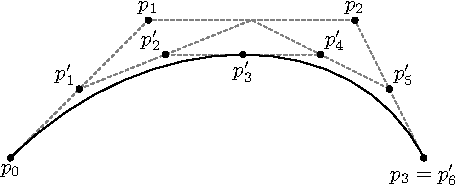
\includegraphics{subdivision}
	\caption{A Figure}
	\label{subd}
\end{figure}

\clearpage %% starts a new page and stops trying to place floats such as tables and figures

\section{More Figure Stuff}
You can also scale and rotate figures.
\begin{figure}[h!]

	\centering
	% DO NOT ADD A FILENAME EXTENSION TO THE GRAPHIC FILE
	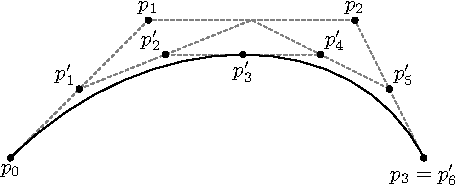
\includegraphics[scale=0.5,angle=180]{subdivision}
	% if your figure shows up not where you want it, it may just be too big to fit. You can use the scale argument to shrink it, e.g. scale=0.85 is 85 percent of the original size.
	\caption{A Smaller Figure, Flipped Upside Down}
	\label{subd2}
\end{figure}

\section{Even More Figure Stuff}
With some clever work you can crop a figure, which is handy if (for instance) your EPS or PDF is a little graphic on a whole sheet of paper. The viewport arguments are the lower-left and upper-right coordinates for the area you want to crop.

\begin{figure}[h!]
	\centering
	% DO NOT ADD A FILENAME EXTENSION TO THE GRAPHIC FILE
	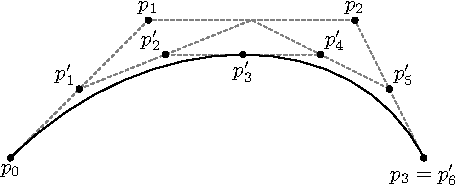
\includegraphics[clip=true, viewport=.0in .0in 1in 1in]{subdivision}
	\caption{A Cropped Figure}
	\label{subd3}
\end{figure}

\subsection{Common Modifications}
The following figure features the more popular changes thesis students want to their figures. This information is also on the web at \url{web.reed.edu/cis/help/latex/graphics.html}.
%\renewcommand{\thefigure}{0.\arabic{figure}} 	% Renumbers the figure to the type 0.x
%\addtocounter{figure}{4} 						% starts the figure numbering at 4
\begin{figure}[htbp]
	\begin{center}
		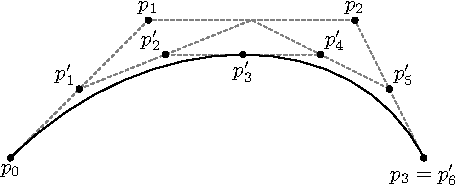
\includegraphics[scale=0.5]{subdivision}
		\caption[Subdivision of arc segments]{\footnotesize{Subdivision of arc segments. You can see that $ p_3 = p_6^\prime$.}} %the special ToC caption is in square brackets. The \footnotesize makes the figure caption smaller
		\label{barplot}
	\end{center}
\end{figure}

\chapter*{Conclusion}
\addcontentsline{toc}{chapter}{Conclusion}
\chaptermark{Conclusion}
\markboth{Conclusion}{Conclusion}
\setcounter{chapter}{4}
\setcounter{section}{0}

Here's a conclusion, demonstrating the use of all that manual incrementing and table of contents adding that has to happen if you use the starred form of the chapter command. The deal is, the chapter command in \LaTeX\ does a lot of things: it increments the chapter counter, it resets the section counter to zero, it puts the name of the chapter into the table of contents and the running headers, and probably some other stuff.

So, if you remove all that stuff because you don't like it to say ``Chapter 4: Conclusion'', then you have to manually add all the things \LaTeX\ would normally do for you. Maybe someday we'll write a new chapter macro that doesn't add ``Chapter X'' to the beginning of every chapter title.

\section{More info}
And here's some other random info: the first paragraph after a chapter title or section head \emph{shouldn't be} indented, because indents are to tell the reader that you're starting a new paragraph. Since that's obvious after a chapter or section title, proper typesetting doesn't add an indent there.


%If you feel it necessary to include an appendix, it goes here.
\appendix
\chapter{The First Appendix}
\chapter{The Second Appendix, for Fun}


%This is where endnotes are supposed to go, if you have them.
%I have no idea how endnotes work with LaTeX.

\backmatter % backmatter makes the index and bibliography appear properly in the t.o.c...

% if you're using bibtex, the next line forces every entry in the bibtex file to be included
% in your bibliography, regardless of whether or not you've cited it in the thesis.
\nocite{*}

% Rename my bibliography to be called "Works Cited" and not "References" or ``Bibliography''
% \renewcommand{\bibname}{Works Cited}

%    \bibliographystyle{bsts/mla-good} % there are a variety of styles available;
%  \bibliographystyle{plainnat}
% replace ``plainnat'' with the style of choice. You can refer to files in the bsts or APA
% subfolder, e.g.
\bibliographystyle{APA/apa-good}  % or
\bibliography{thesis}
% Comment the above two lines and uncomment the next line to use biblatex-chicago.
%\printbibliography[heading=bibintoc]

% Finally, an index would go here... but it is also optional.
\end{document}
